\pdfminorversion=4
\documentclass[10pt]{beamer}\usepackage[]{graphicx}\usepackage[]{color}
%% maxwidth is the original width if it is less than linewidth
%% otherwise use linewidth (to make sure the graphics do not exceed the margin)
\makeatletter
\def\maxwidth{ %
  \ifdim\Gin@nat@width>\linewidth
    \linewidth
  \else
    \Gin@nat@width
  \fi
}
\makeatother

\definecolor{fgcolor}{rgb}{0.345, 0.345, 0.345}
\newcommand{\hlnum}[1]{\textcolor[rgb]{0.686,0.059,0.569}{#1}}%
\newcommand{\hlstr}[1]{\textcolor[rgb]{0.192,0.494,0.8}{#1}}%
\newcommand{\hlcom}[1]{\textcolor[rgb]{0.678,0.584,0.686}{\textit{#1}}}%
\newcommand{\hlopt}[1]{\textcolor[rgb]{0,0,0}{#1}}%
\newcommand{\hlstd}[1]{\textcolor[rgb]{0.345,0.345,0.345}{#1}}%
\newcommand{\hlkwa}[1]{\textcolor[rgb]{0.161,0.373,0.58}{\textbf{#1}}}%
\newcommand{\hlkwb}[1]{\textcolor[rgb]{0.69,0.353,0.396}{#1}}%
\newcommand{\hlkwc}[1]{\textcolor[rgb]{0.333,0.667,0.333}{#1}}%
\newcommand{\hlkwd}[1]{\textcolor[rgb]{0.737,0.353,0.396}{\textbf{#1}}}%

\usepackage{framed}
\makeatletter
\newenvironment{kframe}{%
 \def\at@end@of@kframe{}%
 \ifinner\ifhmode%
  \def\at@end@of@kframe{\end{minipage}}%
  \begin{minipage}{\columnwidth}%
 \fi\fi%
 \def\FrameCommand##1{\hskip\@totalleftmargin \hskip-\fboxsep
 \colorbox{shadecolor}{##1}\hskip-\fboxsep
     % There is no \\@totalrightmargin, so:
     \hskip-\linewidth \hskip-\@totalleftmargin \hskip\columnwidth}%
 \MakeFramed {\advance\hsize-\width
   \@totalleftmargin\z@ \linewidth\hsize
   \@setminipage}}%
 {\par\unskip\endMakeFramed%
 \at@end@of@kframe}
\makeatother

\definecolor{shadecolor}{rgb}{.97, .97, .97}
\definecolor{messagecolor}{rgb}{0, 0, 0}
\definecolor{warningcolor}{rgb}{1, 0, 1}
\definecolor{errorcolor}{rgb}{1, 0, 0}
\newenvironment{knitrout}{}{} % an empty environment to be redefined in TeX

\usepackage{alltt}
%% O comando acima foi necessario porque o PDF nao abria no acrobat do
%% windows, dava o erro 131. Provavelmente devido as figuras em
%% PDF. Agora ele gera um PDF versao 1.4, ao inves da versao 1.5

\usetheme[compress]{PaloAlto}
\usecolortheme{sidebartab} % crane

\usepackage[brazilian]{babel}
\usepackage[T1]{fontenc}
\usepackage[utf8]{inputenc}
\usepackage{graphicx}
\usepackage{hyperref}
\usepackage[scaled]{beramono} % truetype: Bistream Vera Sans Mono
%\usepackage{inconsolata}
\usepackage{xfrac}
\usepackage{tikz}
\usepackage{xcolor}
\usepackage{multirow}
\usepackage{multicol}
%\usepackage{paralist}

\setbeamertemplate{footline}[frame number] % mostra o numero dos slides
\setbeamertemplate{navigation symbols}{} % retira a barra de navegacao

\usepackage{xspace}
\providecommand{\eg}{\textit{e.g.}\xspace}
\providecommand{\ie}{\textit{i.e.}\xspace}
\providecommand{\R}{\textsf{R}\xspace}
\newcommand{\mb}[1]{\mathbf{#1}}
\newcommand{\bs}[1]{\boldsymbol{#1}}
\providecommand{\E}{\text{E}}
\providecommand{\Var}{\text{Var}}
\theoremstyle{definition}
\newtheorem*{mydef}{Definição}
\newtheorem*{mythm}{Teorema}

\title{Modelos Lineares Generalizados (MLGs)}
\author[]{Fernando de Pol Mayer}
\institute[UFPR]{Laboratório de Estatística e Geoinformação (LEG) \\
  Departamento de Estatística (DEST) \\
  Universidade Federal do Paraná (UFPR)}
\date{}
\logo{
\includegraphics[width=1.6cm]{img/ufpr-logo.png}}
\titlegraphic{
\includegraphics[width=1cm]{img/CC_by-nc-sa_88x31.png}\\
  \tiny
  \href{https://creativecommons.org/licenses/by-nc-sa/4.0/deed.pt_BR}{Este
    conteúdo está disponível por meio da Licença Creative Commons 4.0
    (Atribuição/NãoComercial/PartilhaIgual)}}

\AtBeginSection[]
{
  \begin{frame}
    \frametitle{Plano de aula}
    \tableofcontents[currentsection]
  \end{frame}
}

\AtBeginSubsection[]
{
  \begin{frame}
    \frametitle{Plano de aula}
    \tableofcontents[currentsection,currentsubsection]
  \end{frame}
}
\IfFileExists{upquote.sty}{\usepackage{upquote}}{}
\begin{document}





\begin{frame}
\maketitle
%\titlepage
\end{frame}

\begin{frame}{Sumário}
\tableofcontents
\end{frame}

\section[Introdução]{Introdução}

\begin{frame}[fragile]{Base de dados}
\begin{knitrout}\footnotesize
\definecolor{shadecolor}{rgb}{0.969, 0.969, 0.969}\color{fgcolor}\begin{kframe}
\begin{alltt}
\hlstd{dados} \hlkwb{<-} \hlkwd{read.table}\hlstd{(}\hlstr{"dados/crabs.csv"}\hlstd{,} \hlkwc{header} \hlstd{= T,}
                    \hlkwc{sep} \hlstd{=} \hlstr{";"}\hlstd{,} \hlkwc{dec} \hlstd{=} \hlstr{","}\hlstd{)}
\hlkwd{str}\hlstd{(dados)}
\end{alltt}
\begin{verbatim}
'data.frame':	156 obs. of  7 variables:
 $ especie: Factor w/ 2 levels "azul","laranja": 1 1 1 1 1 1 1 1 1 1 ...
 $ sexo   : Factor w/ 2 levels "F","M": 2 2 2 2 2 2 2 2 2 2 ...
 $ FL     : num  8.1 8.8 9.2 9.6 10.8 11.6 11.8 12.3 12.6 12.8 ...
 $ RW     : num  6.7 7.7 7.8 7.9 9 9.1 10.5 11 10 10.9 ...
 $ CL     : num  16.1 18.1 19 20.1 23 24.5 25.2 26.8 27.7 27.4 ...
 $ CW     : num  19 20.8 22.4 23.1 26.5 28.4 29.3 31.5 31.7 31.5 ...
 $ BD     : num  7 7.4 7.7 8.2 9.8 10.4 10.3 11.4 11.4 11 ...
\end{verbatim}
\end{kframe}
\end{knitrout}
\end{frame}

\section{Testes de hipótese}

\begin{frame}[fragile]{Testes de hipótese}{Teste-t
    para uma amostra}
\begin{knitrout}\footnotesize
\definecolor{shadecolor}{rgb}{0.969, 0.969, 0.969}\color{fgcolor}\begin{kframe}
\begin{alltt}
\hlkwd{hist}\hlstd{(dados}\hlopt{$}\hlstd{CL,} \hlkwc{main} \hlstd{=} \hlstr{""}\hlstd{,} \hlkwc{ylab} \hlstd{=} \hlstr{"Frequência absoluta"}\hlstd{,}
     \hlkwc{xlab} \hlstd{=} \hlstr{"Comprimento da carapaça (mm)"}\hlstd{,} \hlkwc{col} \hlstd{=} \hlstr{"grey"}\hlstd{)}
\end{alltt}
\end{kframe}

{\centering 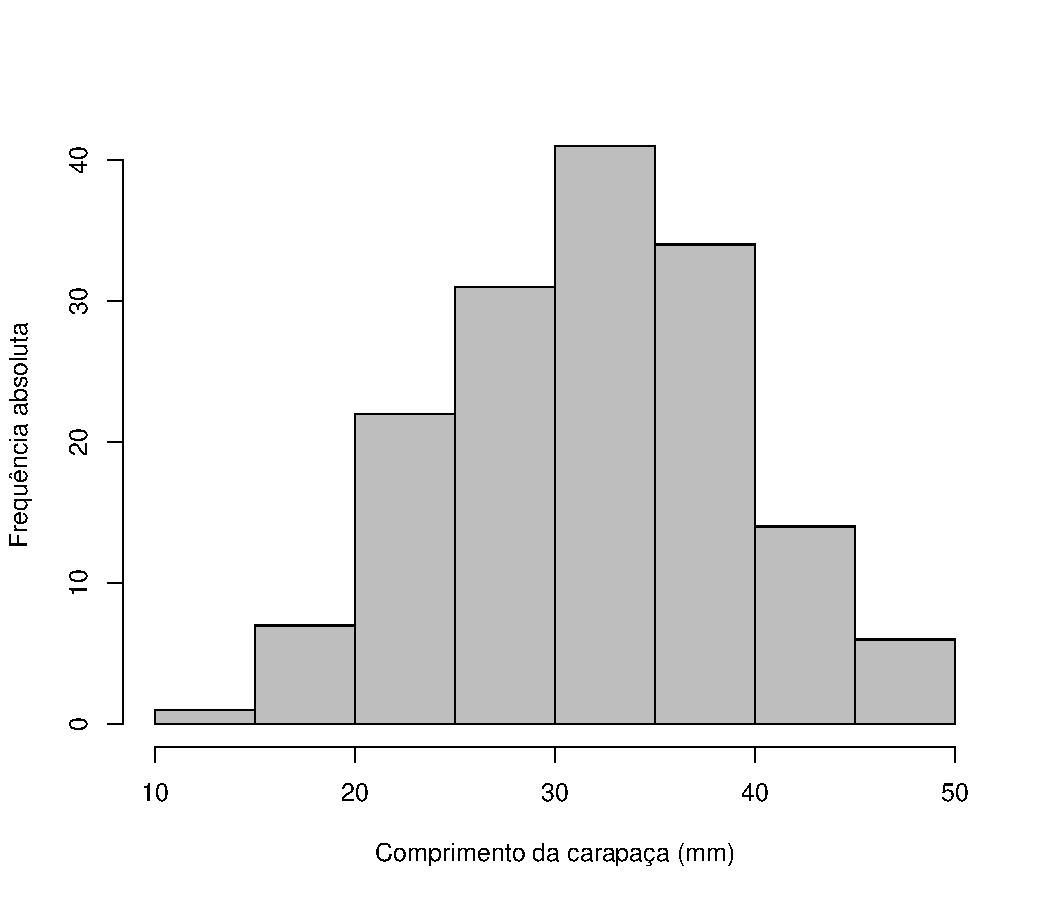
\includegraphics[width=.8\textwidth]{figure/unnamed-chunk-2-1} 

}



\end{knitrout}
\end{frame}

\begin{frame}[fragile]{Testes de hipótese}{Teste-t
    para uma amostra}
Procedimentos gerais para um teste de hipótese
\begin{enumerate}[(1)]
\item Definir a hipótese nula ($H_0$) e a alternativa ($H_1$)
\item Definir um nível de \textbf{significância} $\alpha$ (ex.: $\alpha
  = 0,05$), que irá determinar o nível de \textbf{confiança}
  $100(1-\alpha)\%$ do teste
\item Determinar a \textbf{região de rejeição} com base no nível de
  significância $\rightarrow$ $t_{crit}$
\item Calcula a \textbf{estatística de teste}, sob a hipótese nula
  \begin{equation*}
    t_{calc} = \frac{\bar{x} - \mu_0}{s/\sqrt{n}}
  \end{equation*}
\item Rejeitar a hipótese nula se a estatística de teste calculada
  estiver dentro da região de rejeição ($t_{calc} > t_{crit}$)
  \begin{itemize}
  \item Alternativamente, calcula-se o p-valor, que é a probabilidade de
    se obter um valor de $t$ igual ou maior do que $t_{calc}$
  \end{itemize}
\end{enumerate}
\end{frame}

\begin{frame}[fragile]{Testes de hipótese}{Teste-t para uma
    amostra}
  \begin{itemize}
  \item Testar a hipótese de que a média ($\mu$) de CL é igual a 30 mm
    (com 95\% de confiança)
  \item As hipóteses são
    \begin{align*}
      H_0: \mu = 30 \\
      H_1: \mu \neq 30
    \end{align*}
  \end{itemize}
\end{frame}

\begin{frame}[fragile]{Testes de hipótese}{Teste-t para uma
    amostra}
  Fazendo manualmente
\begin{knitrout}\footnotesize
\definecolor{shadecolor}{rgb}{0.969, 0.969, 0.969}\color{fgcolor}\begin{kframe}
\begin{alltt}
\hlcom{## Dados}
\hlstd{xbarra} \hlkwb{<-} \hlkwd{mean}\hlstd{(dados}\hlopt{$}\hlstd{CL)}
\hlstd{mu0} \hlkwb{<-} \hlnum{30}
\hlstd{dp} \hlkwb{<-} \hlkwd{sd}\hlstd{(dados}\hlopt{$}\hlstd{CL)}
\hlstd{n} \hlkwb{<-} \hlkwd{nrow}\hlstd{(dados)}
\hlcom{# t calculado}
\hlstd{(tcalc} \hlkwb{<-} \hlstd{(xbarra} \hlopt{-} \hlstd{mu0)}\hlopt{/}\hlstd{(dp}\hlopt{/}\hlkwd{sqrt}\hlstd{(n)))}
\end{alltt}
\begin{verbatim}
[1] 3.462731
\end{verbatim}
\begin{alltt}
\hlcom{# t critico (não é apresentado no resultado da função do R)}
\hlkwd{qt}\hlstd{(}\hlnum{0.025}\hlstd{,} \hlkwc{df} \hlstd{= n} \hlopt{-} \hlnum{1}\hlstd{,} \hlkwc{lower.tail} \hlstd{=} \hlnum{FALSE}\hlstd{)}
\end{alltt}
\begin{verbatim}
[1] 1.975387
\end{verbatim}
\begin{alltt}
\hlcom{# valor p (multiplicado por 2 pois o teste é bilateral)}
\hlkwd{pt}\hlstd{(tcalc,} \hlkwc{df} \hlstd{= n} \hlopt{-} \hlnum{1}\hlstd{,} \hlkwc{lower.tail} \hlstd{=} \hlnum{FALSE}\hlstd{)} \hlopt{*} \hlnum{2}
\end{alltt}
\begin{verbatim}
[1] 0.000691346
\end{verbatim}
\end{kframe}
\end{knitrout}
\end{frame}

\begin{frame}[fragile]{Testes de hipótese}{Teste-t para uma
    amostra}
\begin{knitrout}\footnotesize
\definecolor{shadecolor}{rgb}{0.969, 0.969, 0.969}\color{fgcolor}\begin{kframe}
\begin{alltt}
\hlkwd{t.test}\hlstd{(dados}\hlopt{$}\hlstd{CL,} \hlkwc{mu} \hlstd{=} \hlnum{30}\hlstd{,} \hlkwc{alternative} \hlstd{=} \hlstr{"two.sided"}\hlstd{,}
       \hlkwc{conf.level} \hlstd{=} \hlnum{0.95}\hlstd{)}
\end{alltt}
\begin{verbatim}

	One Sample t-test

data:  dados$CL
t = 3.4627, df = 155, p-value = 0.0006913
alternative hypothesis: true mean is not equal to 30
95 percent confidence interval:
 30.86071 33.14698
sample estimates:
mean of x 
 32.00385 
\end{verbatim}
\end{kframe}
\end{knitrout}
\end{frame}

\begin{frame}[fragile]{Testes de hipótese}{Teste-t para uma
    amostra}
\textbf{Detalhe:} O teste pode ser armazenado em um objeto para futuras
referências
\begin{knitrout}\footnotesize
\definecolor{shadecolor}{rgb}{0.969, 0.969, 0.969}\color{fgcolor}\begin{kframe}
\begin{alltt}
\hlstd{teste} \hlkwb{<-} \hlkwd{t.test}\hlstd{(dados}\hlopt{$}\hlstd{CL,} \hlkwc{mu} \hlstd{=} \hlnum{30}\hlstd{,} \hlkwc{alternative} \hlstd{=} \hlstr{"two.sided"}\hlstd{,}
                \hlkwc{conf.level} \hlstd{=} \hlnum{0.95}\hlstd{)}
\hlkwd{names}\hlstd{(teste)}
\end{alltt}
\begin{verbatim}
[1] "statistic"   "parameter"   "p.value"     "conf.int"   
[5] "estimate"    "null.value"  "alternative" "method"     
[9] "data.name"  
\end{verbatim}
\begin{alltt}
\hlstd{teste}\hlopt{$}\hlstd{statistic}
\end{alltt}
\begin{verbatim}
       t 
3.462731 
\end{verbatim}
\begin{alltt}
\hlstd{teste}\hlopt{$}\hlstd{p.value}
\end{alltt}
\begin{verbatim}
[1] 0.000691346
\end{verbatim}
\end{kframe}
\end{knitrout}
\end{frame}

\begin{frame}[fragile]{Testes de hipótese}{Teste-t para duas amostras}
\begin{knitrout}\footnotesize
\definecolor{shadecolor}{rgb}{0.969, 0.969, 0.969}\color{fgcolor}\begin{kframe}
\begin{alltt}
\hlkwd{require}\hlstd{(lattice)} \hlcom{# pacote para gráficos avançados}
\hlkwd{histogram}\hlstd{(}\hlopt{~}\hlstd{CL} \hlopt{|} \hlstd{especie,} \hlkwc{data} \hlstd{= dados)}
\end{alltt}
\end{kframe}

{\centering 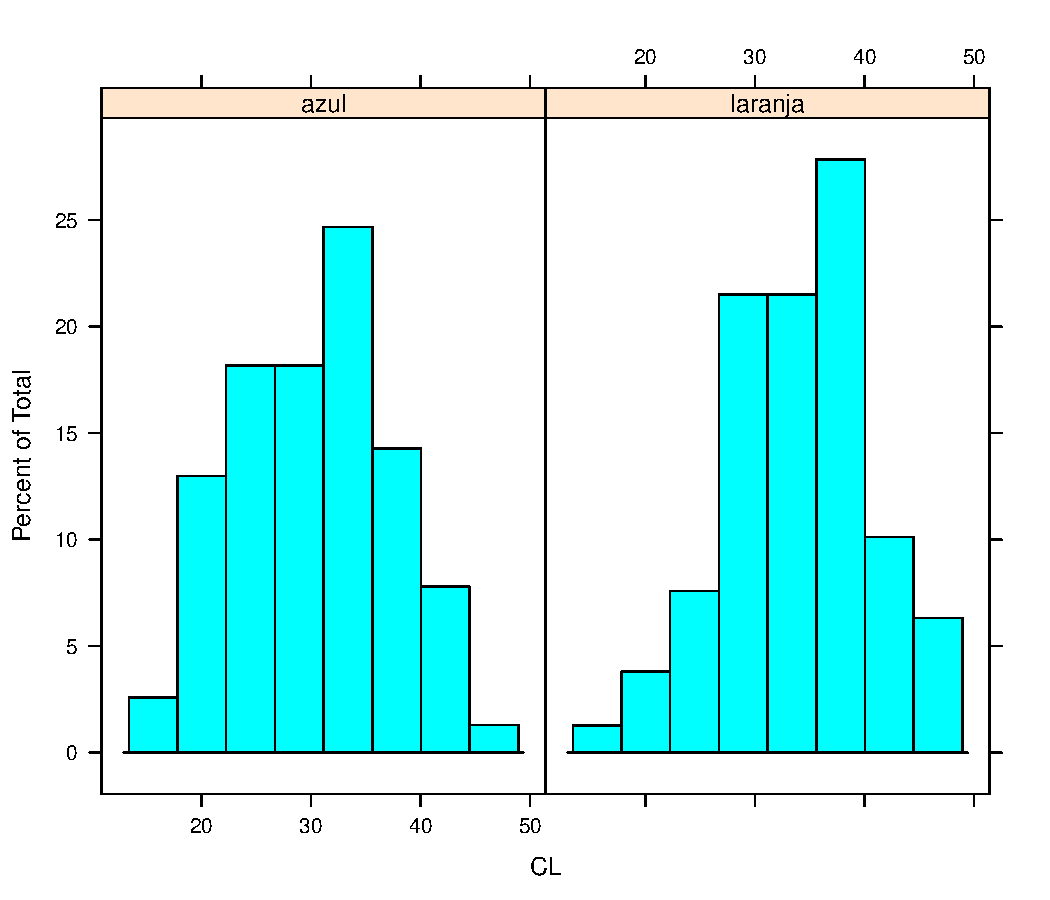
\includegraphics[width=.8\textwidth]{figure/unnamed-chunk-6-1} 

}



\end{knitrout}
\end{frame}

\begin{frame}[fragile]{Testes de hipótese}{Teste-t para duas amostras}
\begin{knitrout}\footnotesize
\definecolor{shadecolor}{rgb}{0.969, 0.969, 0.969}\color{fgcolor}\begin{kframe}
\begin{alltt}
\hlkwd{with}\hlstd{(dados,} \hlkwd{tapply}\hlstd{(CL, especie, summary))}
\end{alltt}
\begin{verbatim}
$azul
   Min. 1st Qu.  Median    Mean 3rd Qu.    Max. 
  14.70   24.60   30.10   29.87   34.50   47.10 

$laranja
   Min. 1st Qu.  Median    Mean 3rd Qu.    Max. 
  16.70   29.40   34.50   34.08   39.25   47.60 
\end{verbatim}
\end{kframe}
\end{knitrout}
Existem evidências de que uma espécie é maior do que a outra?
\end{frame}

\begin{frame}[fragile]{Testes de hipótese}{Teste-t para duas amostras}
  \begin{itemize}
  \item Testar a hipótese de que a \textbf{diferença} entre a média de
    CL da espécie azul ($\mu_A$) e a média de CL da espécie laranja
    ($\mu_L$) é igual a 0 (zero) (com 95\% de confiança)
  \item As hipóteses são
    \begin{align*}
      H_0: \mu_A - \mu_L = 0 \quad \Rightarrow \quad \mu_A = \mu_L \\
      H_1: \mu_A - \mu_L \neq 0 \quad \Rightarrow \quad \mu_A \neq \mu_L
    \end{align*}
  \end{itemize}
\end{frame}

\begin{frame}[fragile]{Testes de hipótese}{Teste-t para duas amostras}
\begin{knitrout}\footnotesize
\definecolor{shadecolor}{rgb}{0.969, 0.969, 0.969}\color{fgcolor}\begin{kframe}
\begin{alltt}
\hlkwd{t.test}\hlstd{(CL} \hlopt{~} \hlstd{especie,} \hlkwc{data} \hlstd{= dados,} \hlkwc{mu} \hlstd{=} \hlnum{0}\hlstd{,}
       \hlkwc{alternative} \hlstd{=} \hlstr{"two.sided"}\hlstd{,} \hlkwc{conf.level} \hlstd{=} \hlnum{0.95}\hlstd{)}
\end{alltt}
\begin{verbatim}

	Welch Two Sample t-test

data:  CL by especie
t = -3.7935, df = 152.73, p-value = 0.0002135
alternative hypothesis: true difference in means is not equal to 0
95 percent confidence interval:
 -6.411592 -2.020366
sample estimates:
   mean in group azul mean in group laranja 
             29.86883              34.08481 
\end{verbatim}
\end{kframe}
\end{knitrout}
Como você faria para calcular a diferença observada das médias de CL
entre as duas espécies?
\end{frame}

\begin{frame}[fragile]{Exercícios}
Com base no objeto \texttt{dados}:
  \begin{enumerate}[(1)]
  \item Faça um histograma de CW
  \item Com base no histograma, construa uma hipótese para a média de CW
    \begin{enumerate}[(a)]
    \item Teste a igualdade dessa hipótese
    \item Teste uma desigualdade dessa hipótese
    \end{enumerate}
    Em ambos os casos use um nível de confiança de 90\%, e escreva uma
    frase com a sua conclusão.
  \item Faça um histograma de CW para cada sexo
  \item Com base nesses histogramas, construa uma hipótese para a
    diferença média de CW entre os sexos
    \begin{enumerate}[(a)]
    \item Teste a igualdade dessa hipótese
    \item Teste uma desigualdade dessa hipótese
    \end{enumerate}
    Em ambos os casos use um nível de confiança de 90\%, e escreva uma
    frase com a sua conclusão.
  \end{enumerate}
\end{frame}

\section{Regressão e correlação}

\begin{frame}[fragile]{Regressão e correlação}
Vamos analisar a relação que existe entre CL e CW
\begin{knitrout}\footnotesize
\definecolor{shadecolor}{rgb}{0.969, 0.969, 0.969}\color{fgcolor}\begin{kframe}
\begin{alltt}
\hlkwd{plot}\hlstd{(CW} \hlopt{~} \hlstd{CL,} \hlkwc{data} \hlstd{= dados)}
\end{alltt}
\end{kframe}

{\centering 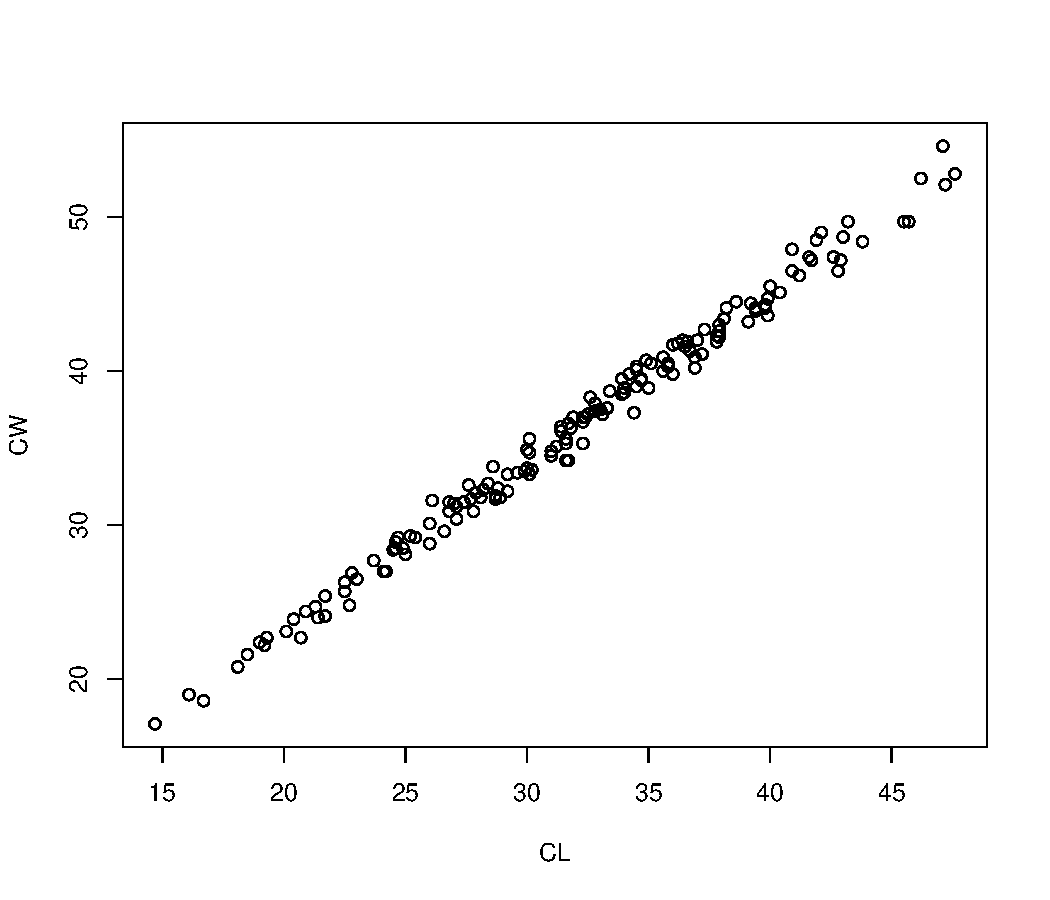
\includegraphics[width=.6\textwidth]{figure/unnamed-chunk-9-1} 

}



\end{knitrout}
\end{frame}

\begin{frame}[fragile]{Regressão e correlação}
  Um \textbf{modelo linear} entre duas variáveis $X$ e $Y$, é definido
  matematicamente como uma equação com dois parâmetros desconhecidos,
  \begin{equation*}
    Y = \beta_0 + \beta_1 X
  \end{equation*}
  A \textbf{análise de regressão} é a técnica estatística que analisa as
  relações existentes entre uma única variável \textbf{dependente}, e
  uma ou mais variáveis \textbf{independentes} \\~\\
  O objetivo é estudar as relações entre as variáveis, a partir de um
  \textbf{modelo matemático}, permitindo \textbf{estimar} o valor de uma
  variável a partir da outra
  \begin{itemize}
  \item Exemplo: sabendo a altura podemos determinar o peso de uma
    pessoa, se conhecemos os parâmetros do modelo anterior
  \end{itemize}
\end{frame}

\begin{frame}[fragile]{Regressão linear}
  O problema da análise de regressão consiste em definir a
  \textbf{forma} de relação existente entre as variáveis. \\~\\
  Por exemplo, podemos ter as seguintes relações
  \begin{align*}
    Y &= \beta_0 + \beta_1 X &\qquad \text{linear} \\
    Y &= \beta_0 X^{\beta_1} &\qquad \text{potência} \\
    Y &= \beta_0 e^{\beta_1 X} &\qquad \text{exponencial} \\
    Y &= \beta_0 + \beta_1 X + \beta_2 X^2 &\qquad \text{polinomial} \\
  \end{align*}
  Em todos os casos, a variável \textbf{dependente} é $Y$, aquela que
  será \textbf{predita} a partir da relação e da variável
  \textbf{independente} $X$
\end{frame}

\subsection{Regressão}

\begin{frame}[fragile]{Regressão linear}
  Em uma \textbf{análise de regressão linear} consideraremos apenas as
  variáveis que possuem uma \textbf{relação linear} entre si. \\~\\
  Uma análise de regressão linear \textbf{múltipla} pode associar $k$
  variáveis independentes ($X$) para ``explicar'' uma única variável
  dependente ($Y$),
  \begin{equation*}
    Y = \beta_0 + \beta_1 X_1 + \beta_2 X_2 + \cdots + \beta_k X_k + e
  \end{equation*}
  Uma análise de regressão linear \textbf{simples} associa uma única
  variável independente ($X$) com uma variável dependente ($Y$),
  \begin{equation*}
    Y = \beta_0 + \beta_1 X + e
  \end{equation*}
\end{frame}

\begin{frame}[fragile]{Regressão linear}
  Assim, dados $n$ pares de valores, $(X_1, Y_1), (X_2, Y_2), \ldots,
  (X_n, Y_n)$, se for admitido que $Y$ é função linear de $X$, pode-se
  estabelecer uma regressão linear simples, cujo modelo estatístico é
  \begin{equation*}
    Y_i = \beta_0 + \beta_1 X_i + e_i, \quad i = 1, 2, \ldots, n
  \end{equation*}
  onde:
  \begin{itemize}
  \item $Y$ é a variável \textbf{resposta} (ou \textbf{dependente})
  \item $X$ é a variável \textbf{explicativa} (ou \textbf{independente})
  \item $\beta_0$ é o \textbf{intercepto} da reta (valor de $Y$ quando
    $X = 0$)
    %% melhorar aqui: beta1 eh tg \alpha, onde \alpha eh o angulo
    %% ver se eh possivel calcular por trigonometria
  \item $\beta_1$ é o \textbf{coeficiente angular} da reta
    (\textbf{efeito} de $X$ sobre $Y$)
  \item $e_i \sim \text{N}(0, \sigma^2)$ é o \textbf{erro}, ou
    \textbf{desvio}, ou \textbf{resíduo}
  \end{itemize}
  O problema agora consiste em \textbf{estimar} os parâmetros $\beta_0$
  e $\beta_1$. \\~\\
\end{frame}

\begin{frame}[fragile]{Regressão linear}
  \textbf{Interpretação dos parâmetros:} \\~\\
  $\beta_0$ representa o ponto onde a reta corta o eixo $Y$ (na maioria
  das vezes não possui interpretação prática) \\~\\
  $\beta_1$ representa a variabilidade em $Y$ causada pelo aumento de
  uma unidade em $X$. Além disso,
  \begin{itemize}
  \item $\beta_1 > 0$ mostra que com o aumento de $X$, também há um
    aumento em $Y$
  \item $\beta_1 = 0$ mostra que \textbf{não há efeito} de $X$ sobre $Y$
  \item $\beta_1 < 0$ mostra que com a aumento de $X$, há uma diminuição
    em $Y$
  \end{itemize}
  %% tirei pq o beta1 eh muito grande, fica dificil interpretar
%% <<echo=FALSE, pdfcrop=TRUE, out.width=".7\\textwidth", fig.width=6,fig.height=5>>=
%% plot(peso ~ alt, xlab = "Altura (cm)", ylab = "Peso (kg)", pch = 19)
%% abline(m0)
%% beta0 <- round(coef(m0)[1], 2)
%% beta1 <- round(coef(m0)[2], 2)
%% text(x = 1.75, y = 60,
%%      labels = bquote(hat(Y) == .(beta0) + .(beta1) * X))
%% @
\end{frame}

% \subsubsection[Estimação]{Estimação dos parâmetros}

\begin{frame}[fragile]{Estimação dos parâmetros}
  Como através de uma amostra obtemos uma estimativa da verdadeira
  equação de regressão, denominamos
  \begin{equation*}
    \hat{Y}_i = \hat{\beta}_0 + \hat{\beta}_1 X_i
  \end{equation*}
  ou seja, $\hat{Y}_i$ é o valor \textbf{estimado} de $Y_i$, através
  das \textbf{estimativas} de $\beta_0$ e $\beta_1$, que chamaremos de
  $\hat{\beta}_0$ e $\hat{\beta}_1$. \\~\\
  Para cada valor de $Y_i$, temos um valor $\hat{Y}_i$ estimado pela
  equação de regressão,
  \begin{equation*}
    Y_i = \hat{Y}_i + e_i
  \end{equation*}
\end{frame}

\begin{frame}[fragile]{Estimação dos parâmetros}
  Portanto, o erro (ou desvio) de cada observação em relação ao modelo
  adotado será
  \begin{align*}
    e_i &= Y_i - \hat{Y}_i \\
    e_i &= Y_i - (\beta_0 + \beta_1 X_i)
  \end{align*}
  % lembre qe soh colca o chapeu quando iguala a zero depois
  Devemos então adotar um modelo cujos parâmetros $\beta_0$ e
  $\beta_1$, tornem esse diferença a menor possível. \\~\\
  Isso equivale a \textbf{minimizar} a \textbf{soma de quadrados dos
  resíduos} ($SQR$), ou do erro,
  \begin{equation*}
  SQR = \sum_{i=1}^{n} [Y_i - (\beta_0 + \beta_1 X_i)]^2
\end{equation*}
\end{frame}

\begin{frame}[fragile]{Estimação dos parâmetros}
  O método de minimizar a soma de quadrados dos resíduos é denominado de
  \textbf{método dos mínimos quadrados}. \\~\\
  Para se encontrar o ponto mínimo de uma função, temos que obter as
  derivadas parciais em relação a cada parâmetro,
  \begin{align*}
    \frac{\partial SQR}{\partial \beta_0} &= 2 \sum_{i=1}^{n} [Y_i -
    \beta_0 - \beta_1 X_i] (-1) \\
    \frac{\partial SQR}{\partial \beta_1} &= 2 \sum_{i=1}^{n} [Y_i -
    \beta_0 - \beta_1 X_i] (-X_i)
  \end{align*}
  e igualar os resultados a zero
  \begin{equation*}
    \hat{\beta}_0 = \frac{\partial SQR}{\partial \beta_0} = 0 \qquad
    \text{e} \qquad
    \hat{\beta}_1 = \frac{\partial SQR}{\partial \beta_1} = 0
  \end{equation*}
\end{frame}

\begin{frame}[fragile]{Estimação dos parâmetros}
  Dessa forma, chegamos às \textbf{estimativas de mínimos quadrados}
  para os parâmetros $\beta_0$ e $\beta_1$:
  \begin{align*}
    \hat{\beta}_1 &= \frac{\sum_{i=1}^{n} X_iY_i - \frac{\sum_{i=1}^{n}
        X_i \sum_{i=1}^{n} Y_i}{n}}{\sum_{i=1}^{n}X_i^2 -
      \frac{(\sum_{i=1}^{n} X_i)^2}{n}} \\
    & \\
    \hat{\beta_0} &= \bar{Y} - \hat{\beta}_1 \bar{X}
  \end{align*}
  onde
  \begin{align*}
    \bar{Y} = \frac{1}{n} \sum_{i=1}^{n} Y_i \qquad \text{e} \qquad
    \bar{X} = \frac{1}{n} \sum_{i=1}^{n} X_i
  \end{align*}
\end{frame}

\begin{frame}[fragile]{Regressão}
Ajustando um modelo linear no \R
\begin{knitrout}\footnotesize
\definecolor{shadecolor}{rgb}{0.969, 0.969, 0.969}\color{fgcolor}\begin{kframe}
\begin{alltt}
\hlstd{mod} \hlkwb{<-} \hlkwd{lm}\hlstd{(CW} \hlopt{~} \hlstd{CL,} \hlkwc{data} \hlstd{= dados)}
\hlstd{mod}
\end{alltt}
\begin{verbatim}

Call:
lm(formula = CW ~ CL, data = dados)

Coefficients:
(Intercept)           CL  
      1.187        1.097  
\end{verbatim}
\end{kframe}
\end{knitrout}
\end{frame}

\begin{frame}[fragile]{Regressão}{Sumário}
\begin{knitrout}\footnotesize
\definecolor{shadecolor}{rgb}{0.969, 0.969, 0.969}\color{fgcolor}\begin{kframe}
\begin{alltt}
\hlkwd{summary}\hlstd{(mod)}
\end{alltt}
\begin{verbatim}

Call:
lm(formula = CW ~ CL, data = dados)

Residuals:
    Min      1Q  Median      3Q     Max 
-1.7762 -0.5699  0.1098  0.4629  1.8273 

Coefficients:
            Estimate Std. Error t value Pr(>|t|)    
(Intercept) 1.186950   0.285340    4.16 5.28e-05 ***
CL          1.097451   0.008698  126.17  < 2e-16 ***
---
Signif. codes:  0 '***' 0.001 '**' 0.01 '*' 0.05 '.' 0.1 ' ' 1

Residual standard error: 0.7827 on 154 degrees of freedom
Multiple R-squared:  0.9904,	Adjusted R-squared:  0.9904 
F-statistic: 1.592e+04 on 1 and 154 DF,  p-value: < 2.2e-16
\end{verbatim}
\end{kframe}
\end{knitrout}
\end{frame}

\begin{frame}[fragile]{Regressão}{Tabela de Análise de Variância}
\begin{knitrout}\footnotesize
\definecolor{shadecolor}{rgb}{0.969, 0.969, 0.969}\color{fgcolor}\begin{kframe}
\begin{alltt}
\hlkwd{anova}\hlstd{(mod)}
\end{alltt}
\begin{verbatim}
Analysis of Variance Table

Response: CW
           Df Sum Sq Mean Sq F value    Pr(>F)    
CL          1 9752.6  9752.6   15919 < 2.2e-16 ***
Residuals 154   94.3     0.6                      
---
Signif. codes:  0 '***' 0.001 '**' 0.01 '*' 0.05 '.' 0.1 ' ' 1
\end{verbatim}
\end{kframe}
\end{knitrout}
\end{frame}

\begin{frame}[fragile]{Regressão}{Ajuste gráfico}
\begin{knitrout}\footnotesize
\definecolor{shadecolor}{rgb}{0.969, 0.969, 0.969}\color{fgcolor}\begin{kframe}
\begin{alltt}
\hlkwd{plot}\hlstd{(CW} \hlopt{~} \hlstd{CL,} \hlkwc{data} \hlstd{= dados)}
\hlkwd{abline}\hlstd{(mod)}
\hlkwd{plot}\hlstd{(CW} \hlopt{~} \hlstd{CL,} \hlkwc{data} \hlstd{= dados,} \hlkwc{xlim} \hlstd{=} \hlkwd{c}\hlstd{(}\hlnum{0}\hlstd{,}\hlnum{50}\hlstd{),} \hlkwc{ylim} \hlstd{=} \hlkwd{c}\hlstd{(}\hlnum{0}\hlstd{,}\hlnum{55}\hlstd{))}
\hlkwd{abline}\hlstd{(mod)}
\end{alltt}
\end{kframe}

{\centering 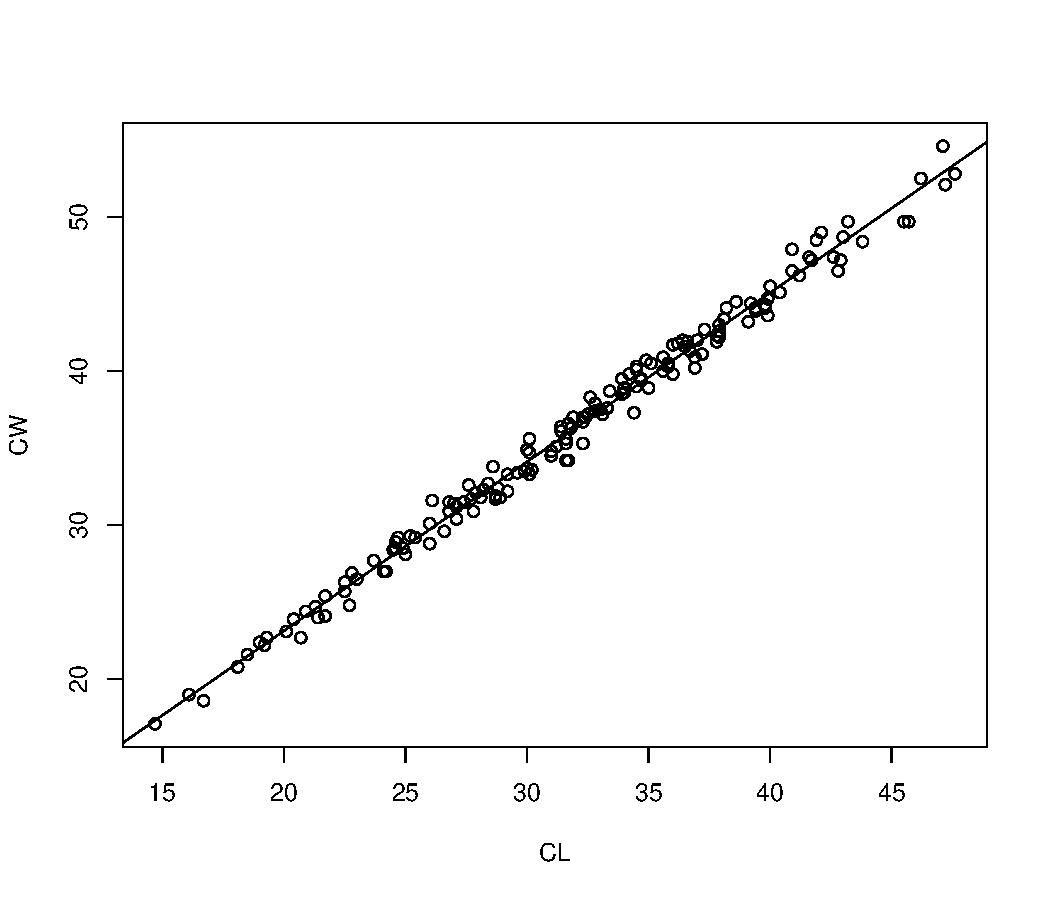
\includegraphics[width=.49\textwidth]{figure/unnamed-chunk-13-1} 
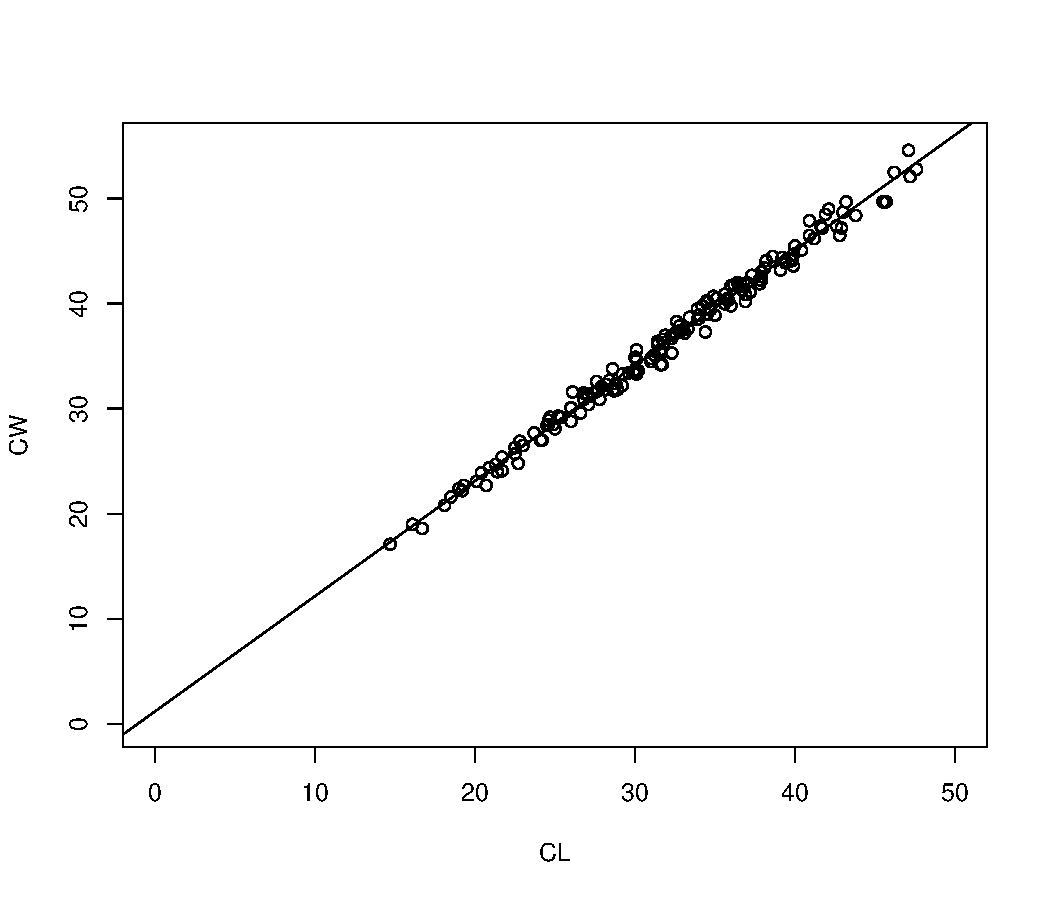
\includegraphics[width=.49\textwidth]{figure/unnamed-chunk-13-2} 

}



\end{knitrout}
\end{frame}

\begin{frame}[fragile]{Regressão}{Análise dos resíduos}
\begin{knitrout}\footnotesize
\definecolor{shadecolor}{rgb}{0.969, 0.969, 0.969}\color{fgcolor}\begin{kframe}
\begin{alltt}
\hlkwd{par}\hlstd{(}\hlkwc{mfrow} \hlstd{=} \hlkwd{c}\hlstd{(}\hlnum{2}\hlstd{,}\hlnum{2}\hlstd{))}
\hlkwd{plot}\hlstd{(mod)}
\hlkwd{par}\hlstd{(}\hlkwc{mfrow} \hlstd{=} \hlkwd{c}\hlstd{(}\hlnum{1}\hlstd{,}\hlnum{1}\hlstd{))}
\end{alltt}
\end{kframe}

{\centering 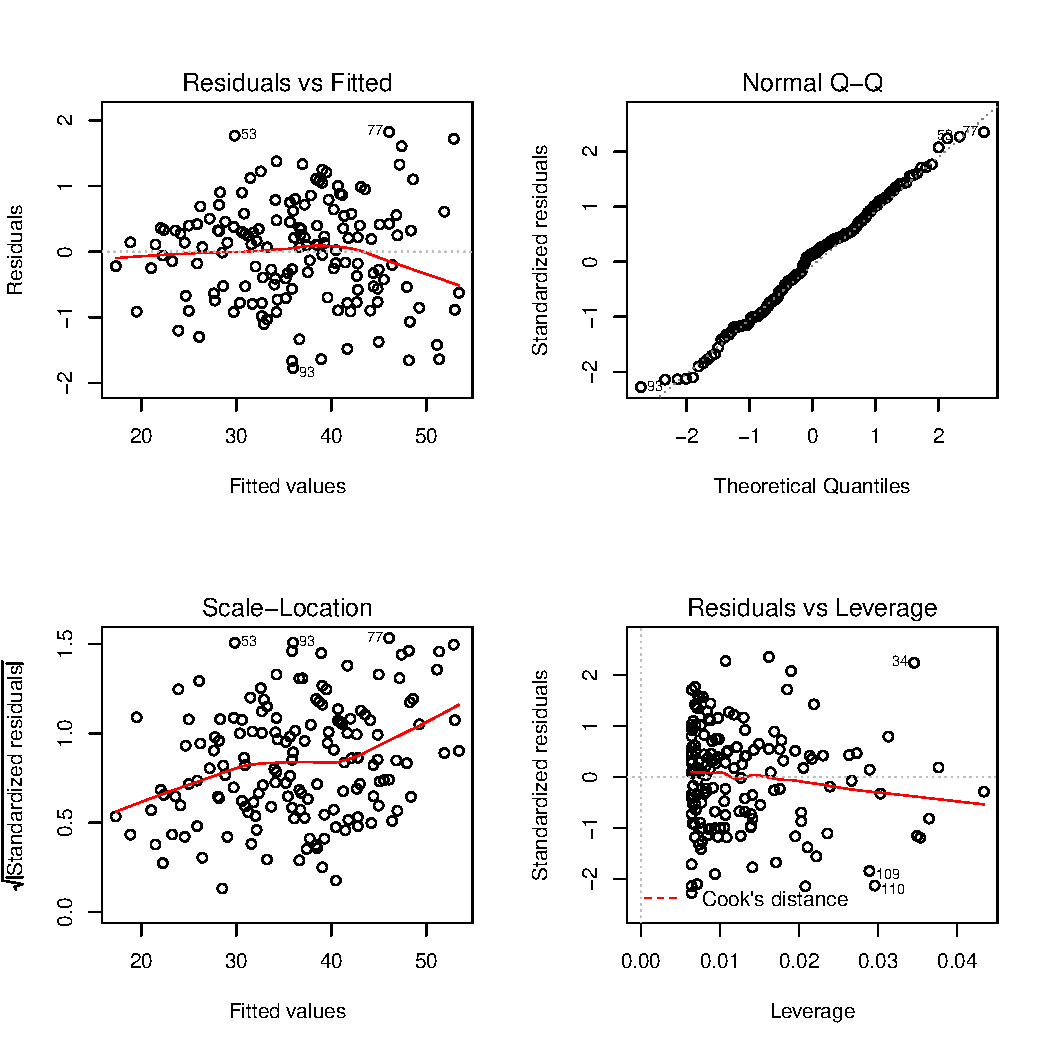
\includegraphics[width=.6\textwidth]{figure/unnamed-chunk-14-1} 

}



\end{knitrout}
\end{frame}

\begin{frame}[fragile]{Regressão}
Acessando os componentes do objeto \texttt{mod}:
\begin{knitrout}\footnotesize
\definecolor{shadecolor}{rgb}{0.969, 0.969, 0.969}\color{fgcolor}\begin{kframe}
\begin{alltt}
\hlkwd{names}\hlstd{(mod)}
\end{alltt}
\begin{verbatim}
 [1] "coefficients"  "residuals"     "effects"      
 [4] "rank"          "fitted.values" "assign"       
 [7] "qr"            "df.residual"   "xlevels"      
[10] "call"          "terms"         "model"        
\end{verbatim}
\begin{alltt}
\hlkwd{names}\hlstd{(}\hlkwd{summary}\hlstd{(mod))}
\end{alltt}
\begin{verbatim}
 [1] "call"          "terms"         "residuals"    
 [4] "coefficients"  "aliased"       "sigma"        
 [7] "df"            "r.squared"     "adj.r.squared"
[10] "fstatistic"    "cov.unscaled" 
\end{verbatim}
\begin{alltt}
\hlkwd{names}\hlstd{(}\hlkwd{anova}\hlstd{(mod))}
\end{alltt}
\begin{verbatim}
[1] "Df"      "Sum Sq"  "Mean Sq" "F value" "Pr(>F)" 
\end{verbatim}
\end{kframe}
\end{knitrout}
\end{frame}

\begin{frame}[fragile]{Regressão}
  Veja que o \texttt{Residual standard error: 0.7827} é o estimador do
  desvio-padrão residual $\hat{\sigma}^{2}_{e} = \frac{\text{SQRes}}{n-2}$,
  ou seja,
\begin{knitrout}\footnotesize
\definecolor{shadecolor}{rgb}{0.969, 0.969, 0.969}\color{fgcolor}\begin{kframe}
\begin{alltt}
\hlkwd{sqrt}\hlstd{(}\hlkwd{anova}\hlstd{(mod)}\hlopt{$}\hlstd{Sum[}\hlnum{2}\hlstd{]}\hlopt{/}\hlkwd{anova}\hlstd{(mod)}\hlopt{$}\hlstd{Df[}\hlnum{2}\hlstd{])}
\end{alltt}
\begin{verbatim}
[1] 0.7827079
\end{verbatim}
\end{kframe}
\end{knitrout}
e que \texttt{F-statistic: 1.592e+04} (15920) é o mesmo valor de
\begin{knitrout}\footnotesize
\definecolor{shadecolor}{rgb}{0.969, 0.969, 0.969}\color{fgcolor}\begin{kframe}
\begin{alltt}
\hlkwd{anova}\hlstd{(mod)}\hlopt{$}\hlstd{F[}\hlnum{1}\hlstd{]}
\end{alltt}
\begin{verbatim}
[1] 15919.11
\end{verbatim}
\end{kframe}
\end{knitrout}
que testa a mesma hipótese da ANOVA. De fato, o valor de $t^2$ para
$\beta_1$ no sumário do modelo é
\begin{knitrout}\footnotesize
\definecolor{shadecolor}{rgb}{0.969, 0.969, 0.969}\color{fgcolor}\begin{kframe}
\begin{alltt}
\hlkwd{summary}\hlstd{(mod)}\hlopt{$}\hlstd{coef[}\hlnum{2}\hlstd{,}\hlnum{3}\hlstd{]}\hlopt{^}\hlnum{2}
\end{alltt}
\begin{verbatim}
[1] 15919.11
\end{verbatim}
\end{kframe}
\end{knitrout}
\end{frame}

\subsection{Correlação}

\begin{frame}[fragile]{Correlação}
  Até agora o interesse estava em estudar qual a influência de uma
  V.A. $X$ sobre uma V.A. $Y$, por meio de uma \textbf{relação linear}. \\~\\
  Assim, em uma análise de regressão é indispensável identificar qual
  variável é dependente. \\~\\
  Na \textbf{análise de correlação} isto não é necessário, pois queremos
  estudar o \textbf{grau de relacionamento} entre as variáveis $X$ e
  $Y$, ou seja, uma medida de \textbf{covariabilidade} entre elas. \\~\\
  A correlação é considerada como uma medida de \textbf{influência
    mútua} entre variáveis, por isso não é necessário especificar quem
  influencia e quem é influenciado.
\end{frame}

\begin{frame}[fragile]{Correlação}
  O \textbf{grau de relação} entre duas variáveis pode ser medido
  através do \textbf{coeficiente de correlação linear} ($r$), dado por
  \begin{equation*}
    r = \frac{\sum_{i=1}^{n} X_iY_i - \frac{\sum_{i=1}^{n}
        X_i \sum_{i=1}^{n} Y_i}{n}}{\sqrt{\sum_{i=1}^{n}X_i^2 -
      \frac{(\sum_{i=1}^{n} X_i)^2}{n}} \cdot \sqrt{\sum_{i=1}^{n}Y_i^2 -
      \frac{(\sum_{i=1}^{n} Y_i)^2}{n}}}
  \end{equation*}
  onde
  \begin{equation*}
    -1 \leq r \leq 1
  \end{equation*}
  Portanto,
  \begin{itemize}
  \item $r=1$ correlação \textbf{positiva} perfeita entre as variáveis
  \item $r=0$ \textbf{não há} correlação entre as variáveis
  \item $r= -1$ correlação \textbf{negativa} perfeita entre as variáveis
  \end{itemize}
\end{frame}

\begin{frame}[fragile]{Correlação}
\begin{knitrout}\footnotesize
\definecolor{shadecolor}{rgb}{0.969, 0.969, 0.969}\color{fgcolor}

{\centering 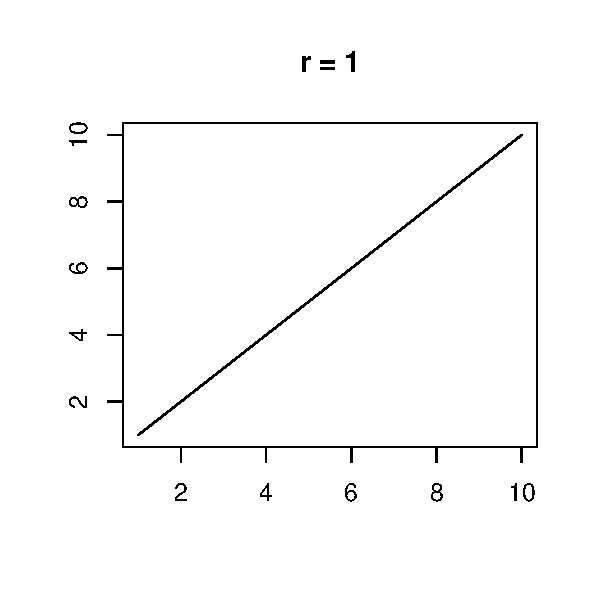
\includegraphics[width=.33\textwidth]{figure/unnamed-chunk-19-1} 
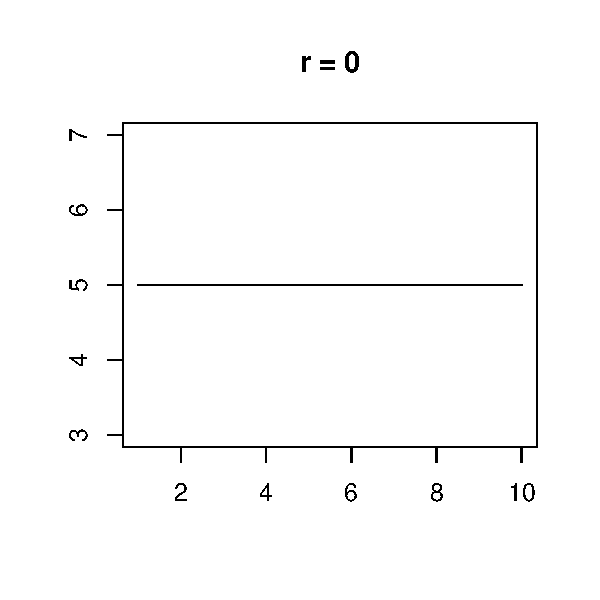
\includegraphics[width=.33\textwidth]{figure/unnamed-chunk-19-2} 
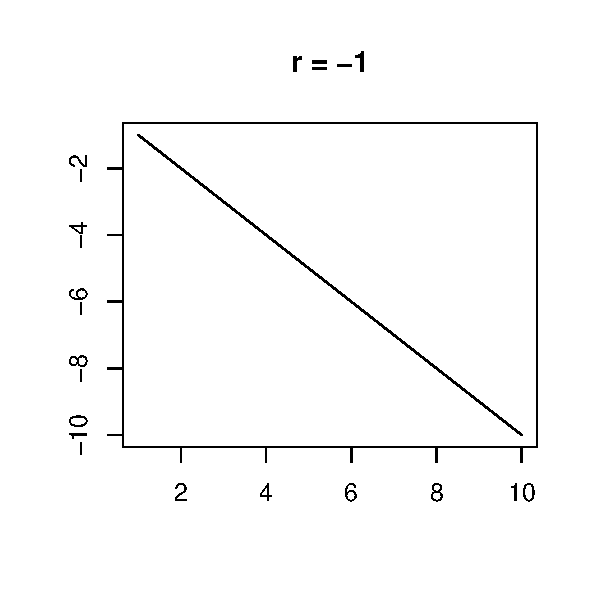
\includegraphics[width=.33\textwidth]{figure/unnamed-chunk-19-3} 

}



\end{knitrout}
\end{frame}

%% Exemplos de que correlacao nao implica em causação

\begin{frame}[fragile]{Correlação}
  O \textbf{coeficiente de determinação} ($r^2$) é o quadrado do
  coeficiente de correlação, por consequência
  \begin{equation*}
    0 \leq r^2 \leq 1
  \end{equation*}
  O $r^2$ nos dá a \textbf{porcentagem de variação em $Y$ que pode ser explicada
  pela variável independente $X$}. \\~\\
  Quanto mais próximo de 1, maior é a explicação da variável $Y$ pela
  variável $X$.
\end{frame}

\begin{frame}[fragile]{Correlação}
\begin{knitrout}\footnotesize
\definecolor{shadecolor}{rgb}{0.969, 0.969, 0.969}\color{fgcolor}

{\centering 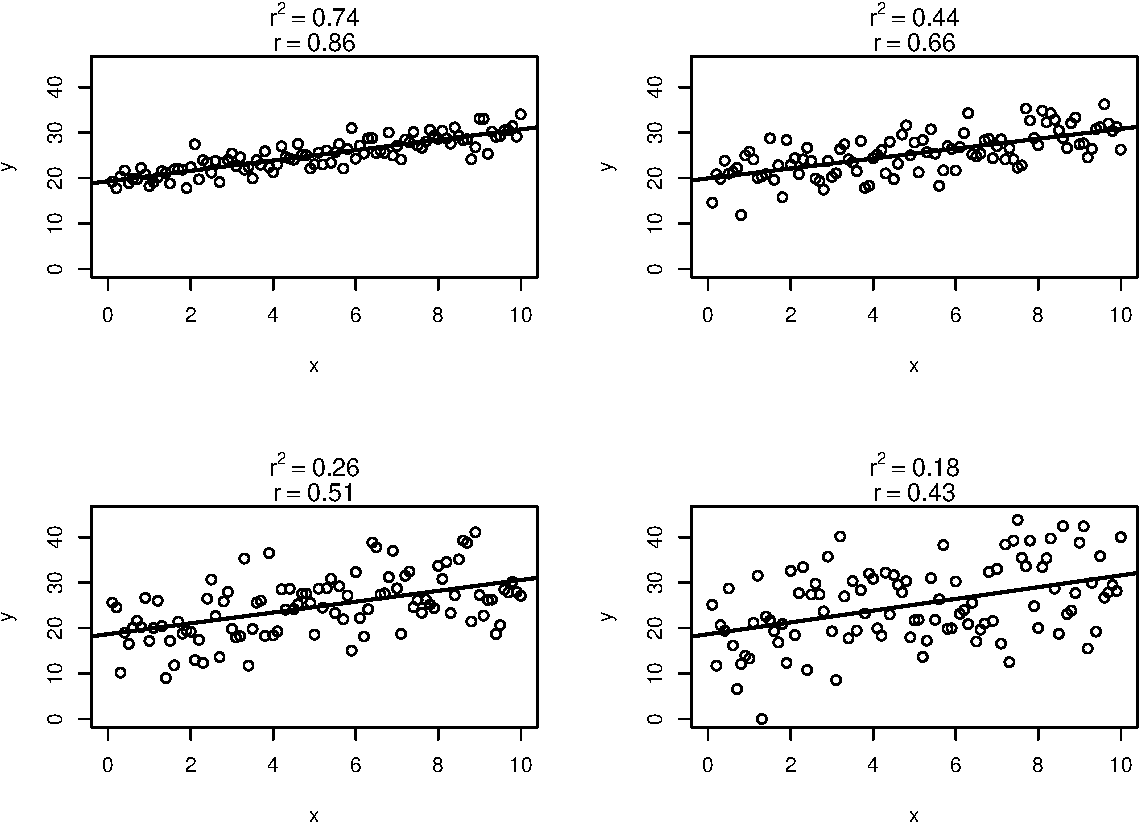
\includegraphics[width=.8\textwidth]{figure/reg-1} 

}



\end{knitrout}
\end{frame}

\begin{frame}[fragile]{Exercícios}
Com as colunas BD e CL do objeto \texttt{dados}
\begin{enumerate}[(1)]
\item Faça um gráfico da relação entre estas variáveis
\item Faça um teste de correlação
\item Ajuste um modelo linear
  \begin{enumerate}[(a)]
  \item Veja o sumário
  \item Ajuste a linha do modelo no gráfico
  \item Verifique os resíduos
  \end{enumerate}
\end{enumerate}
Qual sua conclusão?
\small
\begin{itemize}
\item Existe correlação significativa? De que tipo (positiva, negativa)?
\item O modelo linear descreve bem a relação entre estas duas variáveis
  (verifique com o valor de \verb+Pr(>|t|)+ e do $R^2$)
\item O modelos foi bem ajustado aos dados (observe os resíduos)
\end{itemize}
\end{frame}


\section[ANOVA]{Análise de Variância}

%\begin{frame}[fragile]{Análise de Variância}{Base de dados}
%<<>>=
%## dados <- read.table("crabs.csv", header = T, sep = ";",
%##                     dec = ",")
%## str(dados)
%@
%\end{frame}

\begin{frame}[fragile]{Análise de Variância}
Definição: $y_{ij}$ representa a observação $j$ do grupo $i$;
$\bar{y}_{i}$ é a média do grupo $i$; $\bar{y}$ é a média geral de todas
as observações. As observações podem ser decompostas em
\begin{equation*}
  y_{ij} = \quad \bar{y} \quad + \quad (\bar{y}_{i} - \bar{y}) \quad + \quad
  (y_{ij} - \bar{y}_{i})
\end{equation*}
que corresponde ao modelo
\begin{equation*}
  y_{ij} = \quad \theta \quad + \quad \mu_i \quad + \quad \epsilon_{ij},
  \qquad \epsilon_{ij} \sim N(0, \sigma^2)
\end{equation*}
A hipótese a ser testada de que todos os grupos são iguais (\textit{i.e}
médias iguais) implica que todos os $\mu_{i}$ são iguais:
\begin{align*}
  &H_0: \mu_1 = \mu_2 = \cdots = \mu_n \\
  &H_1: \textsf{pelo menos um}\ \mu_i\ \textsf{é diferente dos demais}
\end{align*}
\end{frame}

\begin{frame}[fragile]{Análise de Variância}
Voltando ao exemplo da diferença de CL entre as duas espécies:\\
$\bar{y}_A = 29.87$ e
$\bar{y}_L = 34.08$
\begin{knitrout}\footnotesize
\definecolor{shadecolor}{rgb}{0.969, 0.969, 0.969}\color{fgcolor}\begin{kframe}
\begin{alltt}
\hlkwd{with}\hlstd{(dados,} \hlkwd{tapply}\hlstd{(CL, especie, summary))}
\end{alltt}
\begin{verbatim}
$azul
   Min. 1st Qu.  Median    Mean 3rd Qu.    Max. 
  14.70   24.60   30.10   29.87   34.50   47.10 

$laranja
   Min. 1st Qu.  Median    Mean 3rd Qu.    Max. 
  16.70   29.40   34.50   34.08   39.25   47.60 
\end{verbatim}
\end{kframe}
\end{knitrout}
Média geral $\bar{y} = 32$
\begin{knitrout}\footnotesize
\definecolor{shadecolor}{rgb}{0.969, 0.969, 0.969}\color{fgcolor}\begin{kframe}
\begin{alltt}
\hlkwd{mean}\hlstd{(dados}\hlopt{$}\hlstd{CL)}
\end{alltt}
\begin{verbatim}
[1] 32.00385
\end{verbatim}
\end{kframe}
\end{knitrout}
\end{frame}

\begin{frame}[fragile]{Análise de Variância}
\begin{knitrout}\footnotesize
\definecolor{shadecolor}{rgb}{0.969, 0.969, 0.969}\color{fgcolor}\begin{kframe}
\begin{alltt}
\hlkwd{boxplot}\hlstd{(CL} \hlopt{~} \hlstd{especie,} \hlkwc{data} \hlstd{= dados)}
\hlkwd{abline}\hlstd{(}\hlkwc{h} \hlstd{=} \hlkwd{mean}\hlstd{(dados}\hlopt{$}\hlstd{CL),} \hlkwc{lty} \hlstd{=} \hlnum{2}\hlstd{,} \hlkwc{col} \hlstd{=} \hlstr{"red"}\hlstd{,} \hlkwc{lwd} \hlstd{=} \hlnum{2}\hlstd{)}
\end{alltt}
\end{kframe}

{\centering 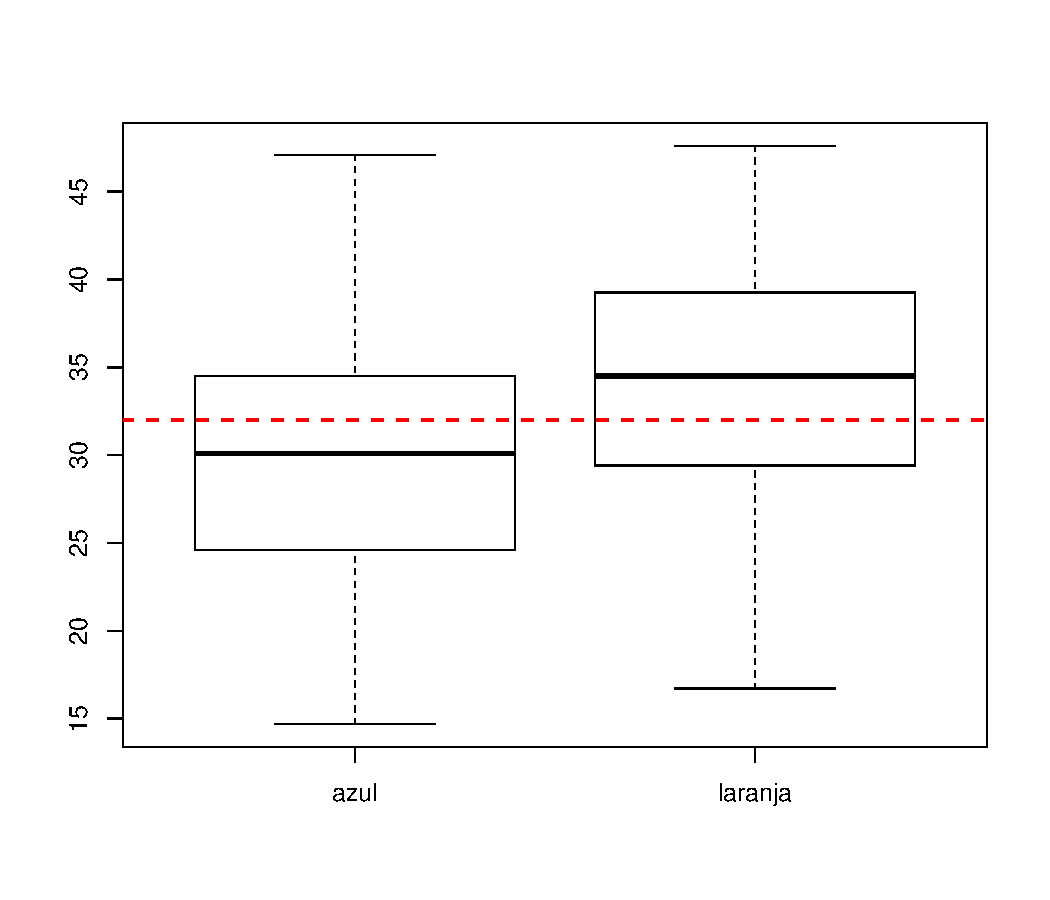
\includegraphics[width=.6\textwidth]{figure/unnamed-chunk-22-1} 

}



\end{knitrout}
\end{frame}

\begin{frame}[fragile]{Análise de Variância}
Geometricamente
\begin{knitrout}\footnotesize
\definecolor{shadecolor}{rgb}{0.969, 0.969, 0.969}\color{fgcolor}

{\centering 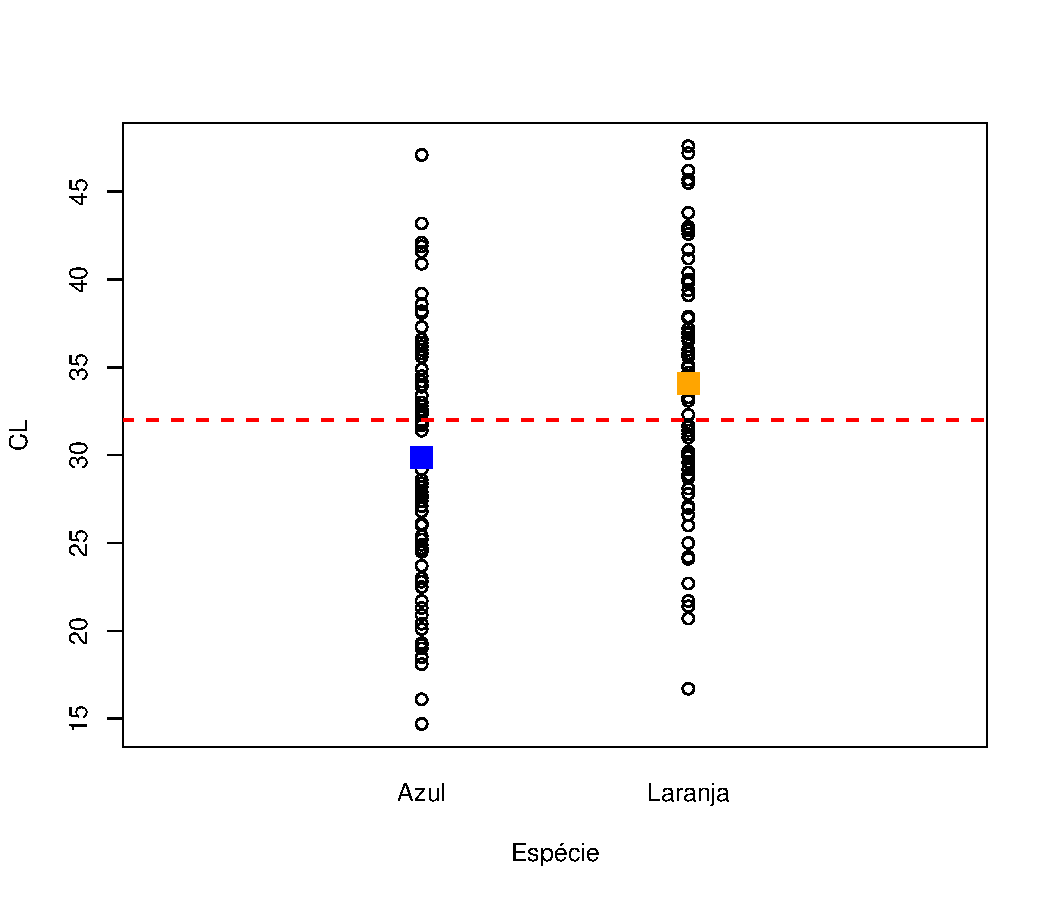
\includegraphics[width=.7\textwidth]{figure/unnamed-chunk-23-1} 

}



\end{knitrout}
\end{frame}

\begin{frame}[fragile]{Análise de Variância}
Podemos ajustar um modelo linear entre CL e espécie
\begin{knitrout}\footnotesize
\definecolor{shadecolor}{rgb}{0.969, 0.969, 0.969}\color{fgcolor}\begin{kframe}
\begin{alltt}
\hlstd{mod} \hlkwb{<-} \hlkwd{lm}\hlstd{(CL} \hlopt{~} \hlstd{especie,} \hlkwc{data} \hlstd{= dados)}
\hlkwd{summary}\hlstd{(mod)}
\end{alltt}
\begin{verbatim}

Call:
lm(formula = CL ~ especie, data = dados)

Residuals:
     Min       1Q   Median       3Q      Max 
-17.3848  -5.0188   0.2732   5.0192  17.2312 

Coefficients:
               Estimate Std. Error t value Pr(>|t|)    
(Intercept)     29.8688     0.7902  37.799  < 2e-16 ***
especielaranja   4.2160     1.1104   3.797  0.00021 ***
---
Signif. codes:  0 '***' 0.001 '**' 0.01 '*' 0.05 '.' 0.1 ' ' 1

Residual standard error: 6.934 on 154 degrees of freedom
Multiple R-squared:  0.08559,	Adjusted R-squared:  0.07966 
F-statistic: 14.42 on 1 and 154 DF,  p-value: 0.0002104
\end{verbatim}
\end{kframe}
\end{knitrout}
\end{frame}

\begin{frame}[fragile]{Análise de Variância}
Ajustando o modelo
\begin{knitrout}\footnotesize
\definecolor{shadecolor}{rgb}{0.969, 0.969, 0.969}\color{fgcolor}

{\centering 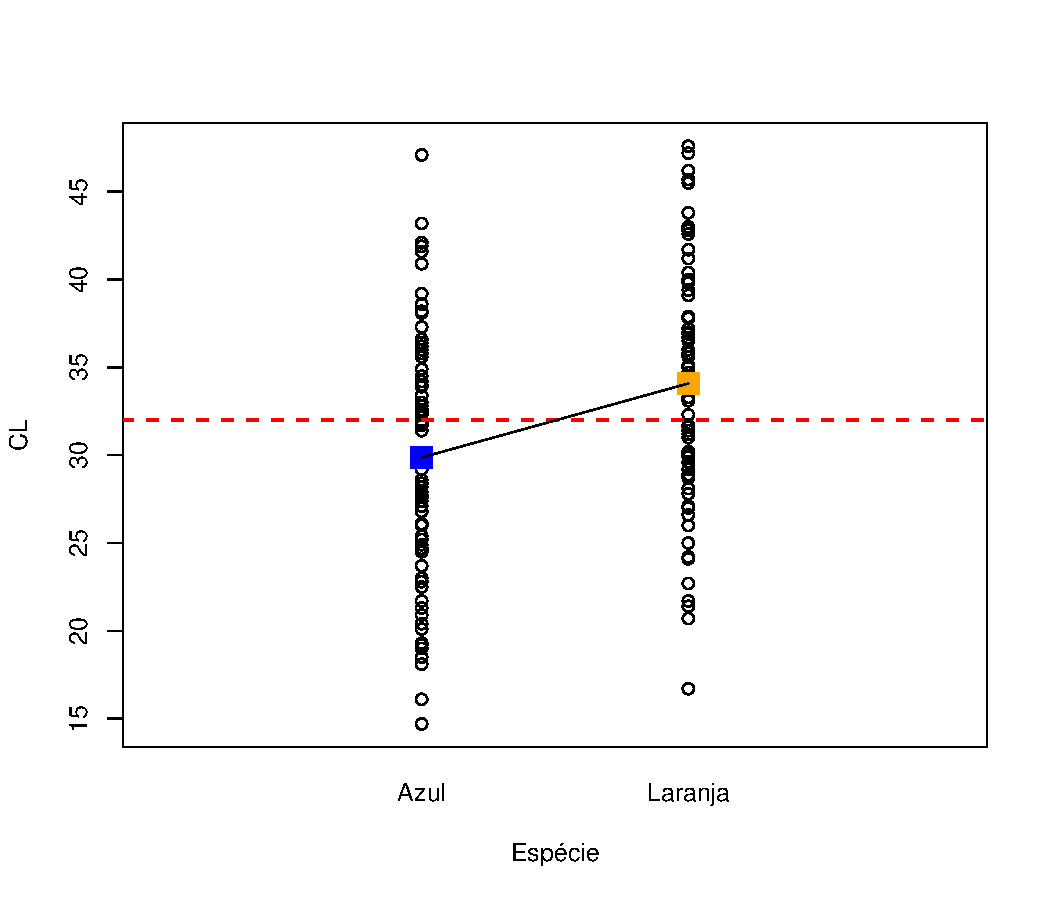
\includegraphics[width=.7\textwidth]{figure/unnamed-chunk-25-1} 

}



\end{knitrout}
\end{frame}

\begin{frame}[fragile]{Análise de Variância}
Você lembra do teste-t feito anteriormente?
\begin{knitrout}\footnotesize
\definecolor{shadecolor}{rgb}{0.969, 0.969, 0.969}\color{fgcolor}\begin{kframe}
\begin{alltt}
\hlstd{teste} \hlkwb{<-} \hlkwd{t.test}\hlstd{(CL} \hlopt{~} \hlstd{especie,} \hlkwc{data} \hlstd{= dados,} \hlkwc{mu} \hlstd{=} \hlnum{0}\hlstd{,}
                \hlkwc{alternative} \hlstd{=} \hlstr{"two.sided"}\hlstd{,} \hlkwc{conf.level} \hlstd{=} \hlnum{0.95}\hlstd{)}
\hlstd{teste}
\end{alltt}
\begin{verbatim}

	Welch Two Sample t-test

data:  CL by especie
t = -3.7935, df = 152.73, p-value = 0.0002135
alternative hypothesis: true difference in means is not equal to 0
95 percent confidence interval:
 -6.411592 -2.020366
sample estimates:
   mean in group azul mean in group laranja 
             29.86883              34.08481 
\end{verbatim}
\end{kframe}
\end{knitrout}
\end{frame}

\begin{frame}[fragile]{Análise de Variância}
Notou a relação?
\begin{knitrout}\footnotesize
\definecolor{shadecolor}{rgb}{0.969, 0.969, 0.969}\color{fgcolor}\begin{kframe}
\begin{alltt}
\hlkwd{summary}\hlstd{(mod)}\hlopt{$}\hlstd{coefficients}
\end{alltt}
\begin{verbatim}
                Estimate Std. Error  t value     Pr(>|t|)
(Intercept)    29.868831  0.7902012 37.79902 8.192364e-80
especielaranja  4.215979  1.1104178  3.79675 2.104221e-04
\end{verbatim}
\begin{alltt}
\hlstd{teste}\hlopt{$}\hlstd{p.value}
\end{alltt}
\begin{verbatim}
[1] 2.135202e-04
\end{verbatim}
\begin{alltt}
\hlstd{teste}\hlopt{$}\hlstd{estimate}
\end{alltt}
\begin{verbatim}
   mean in group azul mean in group laranja 
             29.86883              34.08481 
\end{verbatim}
\begin{alltt}
\hlkwd{unname}\hlstd{(}\hlkwd{diff}\hlstd{(teste}\hlopt{$}\hlstd{estimate))}
\end{alltt}
\begin{verbatim}
[1] 4.215979
\end{verbatim}
\end{kframe}
\end{knitrout}
\end{frame}

\begin{frame}[fragile]{Análise de Variância}
A ANOVA vai testar apenas a hipótese inicial
\begin{align*}
  &H_0: \mu_A = \mu_L \\
  &H_1: \mu_A \neq \mu_L
\end{align*}
\begin{knitrout}\footnotesize
\definecolor{shadecolor}{rgb}{0.969, 0.969, 0.969}\color{fgcolor}\begin{kframe}
\begin{alltt}
\hlkwd{anova}\hlstd{(mod)}
\end{alltt}
\begin{verbatim}
Analysis of Variance Table

Response: CL
           Df Sum Sq Mean Sq F value    Pr(>F)    
especie     1  693.1  693.09  14.415 0.0002104 ***
Residuals 154 7404.3   48.08                      
---
Signif. codes:  0 '***' 0.001 '**' 0.01 '*' 0.05 '.' 0.1 ' ' 1
\end{verbatim}
\end{kframe}
\end{knitrout}
Aqui a única conclusão é de que os $\mu_i$ não são iguais (mas você
não sabe quanto e nem quais!)
\end{frame}

\begin{frame}[fragile]{Análise de Variância}
Se olharmos apenas o resultado da ANOVA, podemos prosseguir com a
análise fazendo um teste \textit{a posteriori} para verificarmos quais
são os grupos que diferem entre si. Um deles é o teste de Tukey
\begin{knitrout}\footnotesize
\definecolor{shadecolor}{rgb}{0.969, 0.969, 0.969}\color{fgcolor}\begin{kframe}
\begin{alltt}
\hlstd{mod.anova} \hlkwb{<-} \hlkwd{aov}\hlstd{(CL} \hlopt{~} \hlstd{especie,} \hlkwc{data} \hlstd{= dados)}
\hlkwd{TukeyHSD}\hlstd{(mod.anova)}
\end{alltt}
\begin{verbatim}
  Tukey multiple comparisons of means
    95% family-wise confidence level

Fit: aov(formula = CL ~ especie, data = dados)

$especie
                 diff      lwr      upr     p adj
laranja-azul 4.215979 2.022362 6.409596 0.0002104
\end{verbatim}
\end{kframe}
\end{knitrout}
\end{frame}

\begin{frame}[fragile]{Análise de Variância}
Porque então fazer uma ANOVA??? \\~\\
\begin{itemize}
\item Quando formos comparar a média de mais de 2 grupos
\item Não é possível fazer um teste-t para mais de 2 grupos
\item Por exemplo, com 3 grupos (A, B, C) teríamos que fazer 3
  comparações (A:B, A:C, B:C)
  \begin{itemize}
  \item Com um nível de confiança de 95\% ($\alpha = 0.05$)
    para cada teste, os 3 testes teriam um nível de confiança
    $(1-\alpha)^3$
  \item Portanto $(1-0.05)^3 = (0.95)^3 = 0.85$
  \item Isso implica que quanto mais comparações forem feitas, menor
    será seu nível de confiança no resultado dos testes.
  \end{itemize}
\end{itemize}
\end{frame}

\section[MLGs]{Modelos Lineares Generalizados}

\begin{frame}[fragile]{Modelos Lineares Generalizados}
  Todos os modelos anteriores podem ser classificados como um caso
  particular de uma \textbf{família de modelos} mais geral, denominada
  \textbf{Modelos Lineares Generalizados} (MLGs):
  \begin{center}
    Teste-t $\subset$ ANOVA $\subset$ ANCOVA* $\subset$ ML $\subset$
    ML-MULT* $\subset$ MLG
  \end{center}
  \begin{itemize}
  \item Teste-t: compara uma ou duas médias
  \item ANOVA: compara 2 ou mais médias (fator)
  \item ANCOVA: compara 2 ou mais médias (fator) + variáveis numéricas
  \item ML: regressão de $Y$ (numérico) em função de um único $X$
    (numérico ou fator)
  \item ML-MULT: regressão de $Y$ (numérico) em função de mais de um $X$
    (numéricos ou fatores)
  \item MLG: Similar ao ML-MULT, mas extende o modelo para que $Y$ possa
    ser um fator ou ter uma distribuição diferente da normal.
  \end{itemize}
\end{frame}

\begin{frame}[fragile]{Modelos Lineares Generalizados}
  A seleção de modelos é uma parte importante de toda pesquisa, envolve
  a procura de um modelo o mais simples possível, que descreva
  bem os dados observados. \\~\\
  Na maior parte das situações pode-se pensar na variável resposta ($Y$)
  consistindo de duas partes distintas: \\~\\
  \begin{enumerate}
  \item Um \textbf{componente sistemático}, que é estabelecido durante o
    planejamento do experimento, resultando em modelos de regressão,
    ANOVA ou ANCOVA.
  \item Um \textbf{componente aleatório}, que é estabelecido assim
  que são definidas as medidas a serem feitas, que podem ser contínuas
  ou discretas, exigindo o ajuste de distribuições diferentes.
\end{enumerate}
\end{frame}

\begin{frame}[fragile]{Modelos Lineares Generalizados}
  Matematicamente, e assumindo o modelo clássico de regressão, temos:
  \begin{equation*}
    \mb{Y} = \bs{\mu} + \mb{e}
  \end{equation*}
  onde:
  \begin{itemize}
  \item $Y$ o vetor de dimensão $n \times 1$ da variável
    \textbf{resposta}
  \item $\bs{\mu} = \E(\mb{Y}) = \mb{X}\bs{\beta}$ o \textbf{componente
    sistemático}
  \item $\mb{X}$ é a \textbf{matriz do modelo}, de dimensão $n \times p$
  \item $\bs{\beta} = (\beta_1, \ldots, \beta_p)^{T}$ o vetor de
    parâmetros
  \item $\mb{e} = (e_1, \ldots, e_n)^{T}$ o \textbf{componente
      aleatório} com $e_i \sim \text{N}(0, \sigma^2)$
  \end{itemize}
\end{frame}

\begin{frame}[fragile]{Modelos Lineares Generalizados}
  Em muitos casos, porém, essa estrutura aditiva entre o componente
  sistemático e o componente aleatório não é satisfeita. \\~\\
  Além disso:
  \begin{itemize}
  \item Não há razão para se restringir à estrutura simples dada por
    $\bs{\mu} = \E(\mb{Y}) = \mb{X}\bs{\beta}$ para o componente
    sistemático
  \item Nem sempre a distribuição normal é adequada para o componente
    aleatório
  \item Nem sempre a suposição de homogeneidade de variâncias é atendida
    (e em muitos casos não deve ser mesmo)
  \end{itemize}
\end{frame}

\begin{frame}[fragile]{Modelos Lineares Generalizados}
  Nelder e Wedderburn (1972) propuseram uma teoria unificadora da
  modelagem estatística, a que deram o nome de \textbf{Modelos Lineares
    Generalizados (MLG)}, como uma extensão dos modelos lineares
  clássicos. \\~\\
  Na realidade, eles mostraram que uma série de técnicas comumente
  estudadas separadamente podem ser reunidas sob o nome de Modelos
  Lineares Generalizados. \\~\\
  Os desenvolvimentos que levaram a esta visão geral da modelagem
  estatística, remontam a mais de um século. \\~\\
  Eles mostraram, então, que a maioria dos problemas estatísticos, que
  surgem nas áreas de oceanografia, agricultura, ecologia, economia,
  etc. podem ser formulados, de uma \textbf{maneira unificada}, como
 \textbf{modelos de regressão}.
\end{frame}

\begin{frame}[fragile]{Modelos Lineares Generalizados}
  Os MLGs possuem uma estrutura similar à dos modelos lineares clássicos,
  e podem ser usados quando se tem uma única variável aleatória $Y$, e
  associado a ela um conjunto de variáveis explicativas $X_1, \ldots,
  X_p$ \\~\\
  Para uma amostra de $n$ observações $(y_i, \mb{x}_i)$ em que $\mb{x}_i =
  (x_{i1}, x_{i2}, \ldots, x_{ip})^{T}$ é o vetor coluna de variáveis
  explicativas, o modelo linear generalizado envolve os três
  componentes:
\end{frame}

\begin{frame}[fragile]{Modelos Lineares Generalizados}
\begin{enumerate}
  \item[1)] \textbf{Componente aleatório}: variável resposta do modelo,
    representado por um conjunto de variáveis aleatórias independentes
    $Y_1, \ldots, Y_n$ provenientes de uma \textbf{mesma distribuição}
    que faz parte da \textbf{família exponencial} com médias $\mu_1,
    \ldots, \mu_n$, ou seja,
    \begin{equation*}
      \E(Y_i) = \mu_i, \qquad i = 1, \ldots, n
    \end{equation*}
  \end{enumerate}
\end{frame}

\begin{frame}[fragile]{Modelos Lineares Generalizados}
  \begin{enumerate}
  \item[2)] \textbf{Componente sistemático}: as variáveis explicativas,
    que entram na forma de uma estrutura linear.
    \begin{align*}
      \eta_i &= \beta_0 + \beta_1 x_{i1} + \beta_2 x_{i2} + \cdots +
               \beta_p x_{ip} \\
             &= \sum_{j=1}^{p} \beta_j x_{ij}
    \end{align*}
    Ou, em forma matricial
    \begin{equation*}
      \bs{\eta} = \mb{x}_{i}^{T} \bs{\beta} = \mb{X}\bs{\beta}
    \end{equation*}
    sendo $X = (x_1, \ldots, x_n)^{T}$ a matriz do modelo, $\bs{\beta} =
    (\beta_1, \ldots, \beta_p)^{T}$ o vetor de parâmetros, e $\bs{\eta} =
    (\eta_1, \ldots, \eta_n)^{T}$ o preditor linear.
  \end{enumerate}
\end{frame}

\begin{frame}[fragile]{Modelos Lineares Generalizados}
  \begin{enumerate}
  \item[3)] \textbf{Função de ligação}: função que liga os componentes
    aleatório e sistemático. O modelo liga $\mu_i$ a $\eta_i$ através de
    \begin{equation*}
      \eta_i = g(\mu_i)
    \end{equation*}
    onde $g(\cdot)$ é uma função monótona e diferenciável. Portanto,
    $g(\cdot)$ liga $\E(Y_i)$ com as variáveis explicativas através de
    \begin{equation*}
      g(\mu_i) = \sum_{j=1}^{p} \beta_j x_{ij} \qquad i = 1, \ldots, n
    \end{equation*}
  \end{enumerate}
\end{frame}

\begin{frame}[fragile]{Família exponencial}
  A \textbf{família exponencial} é uma forma geral de definição de
  algumas distribuições de probabilidade. A função (densidade) de
  probabilidade desta família é:
  \begin{equation*}
    f(y_i; \theta_i) = a(\theta_i) b(y_i) \exp{[y_i Q(\theta_i)]}
  \end{equation*}
  Diversas distribuições importantes como: normal, binomial e Poisson
  fazem parte desta família (\ie são casos particulares). \\~\\
  O termo $Q(\theta)$ é chamado de \textbf{parâmetro natural}. \\~\\
  Se a função de ligação for $Q(\theta)$, ou seja,
  \begin{equation*}
    g(\mu_i) = Q(\theta) = \sum_{j=1}^{p} \beta_j x_{ij}
  \end{equation*}
  ela é chamada de \textbf{função de ligação canônica}.
\end{frame}

\begin{frame}[fragile]{Família exponencial}
  \textbf{Exemplo}: Binomial/Bernoulli \\~\\
  A distribuição Bernoulli é um caso particular de uma distribuição
  binomial com $n=1$, e especifica as probabilidades $P(Y=1) = \pi$ e
  $P(Y=0) = 1-\pi$, e $\E(Y) = \pi$. Na famíla exponencial:
  \begin{align*}
    f(y;\pi) &= \pi^y (1-\pi)^{1-y} \\
             &= (1-\pi) \exp{\left[ y \log\frac{\pi}{1-\pi} \right]} \\
             &= a(\theta)b(y) \exp{[y Q(\theta)]}
  \end{align*}
  Portanto, com $\theta = \mu$, $a(\pi) = 1-\pi$, $b(y) = 1$, $Q(\pi) =
  \log[\frac{\pi}{1-\pi}]$, a \textbf{função de ligação canônica} é
  chamada \textit{logit}, e
  \begin{equation*}
    \text{logit}(\pi) = \log\left( \frac{\pi}{1-\pi}  \right) =
    \sum_{j=1}^{p} \beta_j x_{ij}
  \end{equation*}
  é chamada de \textit{regressão logística}.
\end{frame}

\begin{frame}[fragile]{Família exponencial}
  \textbf{Exemplo}: Poisson \\~\\
  A distribuição de Poisson é comumente utilizada para modelar dados de
  contagem. Seja $Y$ uma contagem, e $\mu = \E(Y)$, a função densidade
  de probabilidade na família exponencial fica:
  \begin{align*}
    f(y;\mu) &= \frac{e^{-\mu} \mu^y}{y!} \\
             &= \exp{(-\mu)} \left( \frac{1}{y!} \right) \exp{(y \log
               \mu)} \\
             &= a(\theta)b(y) \exp{[y Q(\theta)]}
  \end{align*}
  Portanto, com $\theta = \mu$, $a(\mu) = \exp{(-\mu)}$, $b(y) = 1/y!$,
  $Q(\mu) = \log \mu$, a \textbf{função de ligação canônica} é o $\log$,
  e
  \begin{equation*}
    g(\mu) = \log \mu = \sum_{j=1}^{p} \beta_j x_{ij}
  \end{equation*}
  que é chamado de \textit{modelo loglinear de Poisson}.
\end{frame}

\begin{frame}[fragile]{Modelos Lineares Generalizados}
  A classe de MLGs inclui também modelos para variáveis respostas
  contínuas. \\~\\
  A distribuição normal faz parte da família exponencial que inclui um
  \textbf{parâmetro de dispersão}, e seu parâmetro natural é a média.
  Portanto,
  \begin{equation*}
    g(\mu) = \mu
  \end{equation*}
  e um modelo de regressão linear simples é um MLG com função de ligação
  \textbf{identidade}.
\end{frame}

\begin{frame}[fragile]{Funções de ligação e tipos de modelo}
  \begin{table}[!h]
    \centering
    \begin{tabular}{p{1.5cm}ccp{2cm}p{1.5cm}}
      \hline
      Componente aleatório & \multicolumn{2}{c}{Link}
      & Componente sistemático & Modelo \\
      \hline
      Normal & Identidade & $\mu$ & Contínuo & Regressão linear \\
      Normal & Identidade & $\mu$ & Categórico & ANOVA \\
      Normal & Identidade & $\mu$ & Ambos & ANCOVA \\
      Binomial & Logit & $\log_{e}\left( \frac{\mu}{1-\mu} \right)$
                               & Ambos & Regressão logística \\
      Poisson & Log & $\log_{e} \mu$ & Ambos & Loglinear \\
      Multinomial & Logit gen. & & Ambos & Multinomial \\
      \hline
    \end{tabular}
  \end{table}
\end{frame}

\begin{frame}[fragile]{Funções de ligação no R}
Distribuições da família exponencial e funções de ligação (P = link
canônico)
\begin{center}
\begin{table}[h!]
\renewcommand{\baselinestretch}{1}
\small\footnotesize\scriptsize
\begin{tabular}{lcccccc}
\hline
Link & \texttt{binomial} & \texttt{poisson} & \texttt{negative} &
\texttt{Gamma} & \texttt{gaussian} & \texttt{inverse}\\
    &       &    & \texttt{binomial} &  &  & \texttt{gaussian} \\
\hline
\texttt{logit} & P & & & & & \\
\texttt{probit} & $\bullet$ & & & & &  \\
\texttt{cloglog} & $\bullet$ & & & & &  \\
\texttt{identity} &  & $\bullet$ & $\bullet$ & $\bullet$ & P & $\bullet$  \\
\texttt{inverse} &  & & & P & $\bullet$ & $\bullet$  \\
\texttt{log} & $\bullet$  & P & P & $\bullet$ & $\bullet$ & $\bullet$  \\
\verb|1/mu^2| & & & & & & P  \\
\texttt{sqrt} & & $\bullet$ & $\bullet$ & & &  \\
\hline
\end{tabular}
\end{table}
\end{center}
\end{frame}

\begin{frame}[fragile]{Modelos Lineares Generalizados}
  Um método tradicional de análise de dados consistia em transformar
  $Y$, para que a variável resposta ficasse com distribuição normal e
  variância constante. \\~\\
  Em MLGs, a escolha de uma função de ligação \textbf{não} é relacionada
  com a escolha do componente aleatório. \\~\\
  Se uma função de ligação é capaz de linearizar a relação entre a média
  e os preditores, então \textbf{não é necessário} que ela também
  estabilize a variância ou produza normalidade. \\~\\
  Isso está relacionado com o processo de ajuste do modelo, que maximiza
  a verossimilhança para a distribuição de $Y$, que não é mais restrita
  à normal.
\end{frame}

\begin{frame}[fragile]{Modelos Lineares Generalizados}
  MLGs fornecem uma \textbf{teoria unificada de modelagem}, que
  compreende os modelos mais importantes para variáveis contínuas e
  discretas. \\~\\
  A estimativa dos parâmetros em MLGs é realizada através de um
  algoritmo que usa uma versão ponderada dos mínimos quadrados,
  \textit{Iteratively Reweighted Least Squares} (IRLS). \\~\\
  A razão de restringir os MLGs à família exponencial para $Y$ é porque
  este mesmo algoritmo se aplica à todos os membros dessa família, para
  qualquer escolha de função de ligação.
\end{frame}

\begin{frame}[fragile]{Modelos Lineares Generalizados}
Para ajustar um MLG usamos a função \texttt{glm()}
\begin{knitrout}\footnotesize
\definecolor{shadecolor}{rgb}{0.969, 0.969, 0.969}\color{fgcolor}\begin{kframe}
\begin{alltt}
\hlstd{mod.glm} \hlkwb{<-} \hlkwd{glm}\hlstd{(CL} \hlopt{~} \hlstd{especie,} \hlkwc{data} \hlstd{= dados,}
               \hlkwc{family} \hlstd{=} \hlkwd{gaussian}\hlstd{(}\hlkwc{link} \hlstd{=} \hlstr{"identity"}\hlstd{))}
\hlkwd{summary}\hlstd{(mod.glm)}
\end{alltt}
\begin{verbatim}

Call:
glm(formula = CL ~ especie, family = gaussian(link = "identity"), 
    data = dados)

Deviance Residuals: 
     Min        1Q    Median        3Q       Max  
-17.3848   -5.0188    0.2732    5.0192   17.2312  

Coefficients:
               Estimate Std. Error t value Pr(>|t|)    
(Intercept)     29.8688     0.7902  37.799  < 2e-16 ***
especielaranja   4.2160     1.1104   3.797  0.00021 ***
---
Signif. codes:  0 '***' 0.001 '**' 0.01 '*' 0.05 '.' 0.1 ' ' 1

(Dispersion parameter for gaussian family taken to be 48.08018)

    Null deviance: 8097.4  on 155  degrees of freedom
Residual deviance: 7404.3  on 154  degrees of freedom
AIC: 1050.9

Number of Fisher Scoring iterations: 2
\end{verbatim}
\end{kframe}
\end{knitrout}
\end{frame}

\begin{frame}[fragile]{Modelos Lineares Generalizados}
  Deviance
\end{frame}

\begin{frame}[fragile]{Modelos Lineares Generalizados}
  Resíduos e diagnósticos
\end{frame}

\begin{frame}[fragile]{Modelos Lineares Generalizados}
  Quando existe mais de uma variável resposta ($Y$)? \\~\\
  \begin{itemize}
  \item Métodos multivariados (restritos à normalidade)
  \item McGLM (\textit{Multivariate covariance Generalized Linear
      Models}) (Bonat e Jorgensen, 2016)
  \end{itemize}

\end{frame}

\begin{frame}[fragile]{Exercícios}
Com o objeto \texttt{dados}
\begin{enumerate}[(1)]
\item Faça um boxplot de CW por sexo
\item Faça um teste-t para testar se existe diferença entre as médias de
  CW para machos e fêmeas
\item Ajuste um modelo linear para testar essa mesma hipótese
\item Faça uma ANOVA e o teste de Tukey
\end{enumerate}
Qual sua conclusão?
\end{frame}

\section{Referências}


\begin{frame}{Referências}
  \begin{itemize}
  \item Agresti, A. \textbf{Categorical data analysis}. John Wiley \&
    Sons. 2002.
  \item Fox, J; Weisberg, S. \textbf{An R companion to applied
      regression}. Sage. 2011.
  \end{itemize}
\end{frame}

\end{document}
